\begin{figure}[ht]
	\centering
	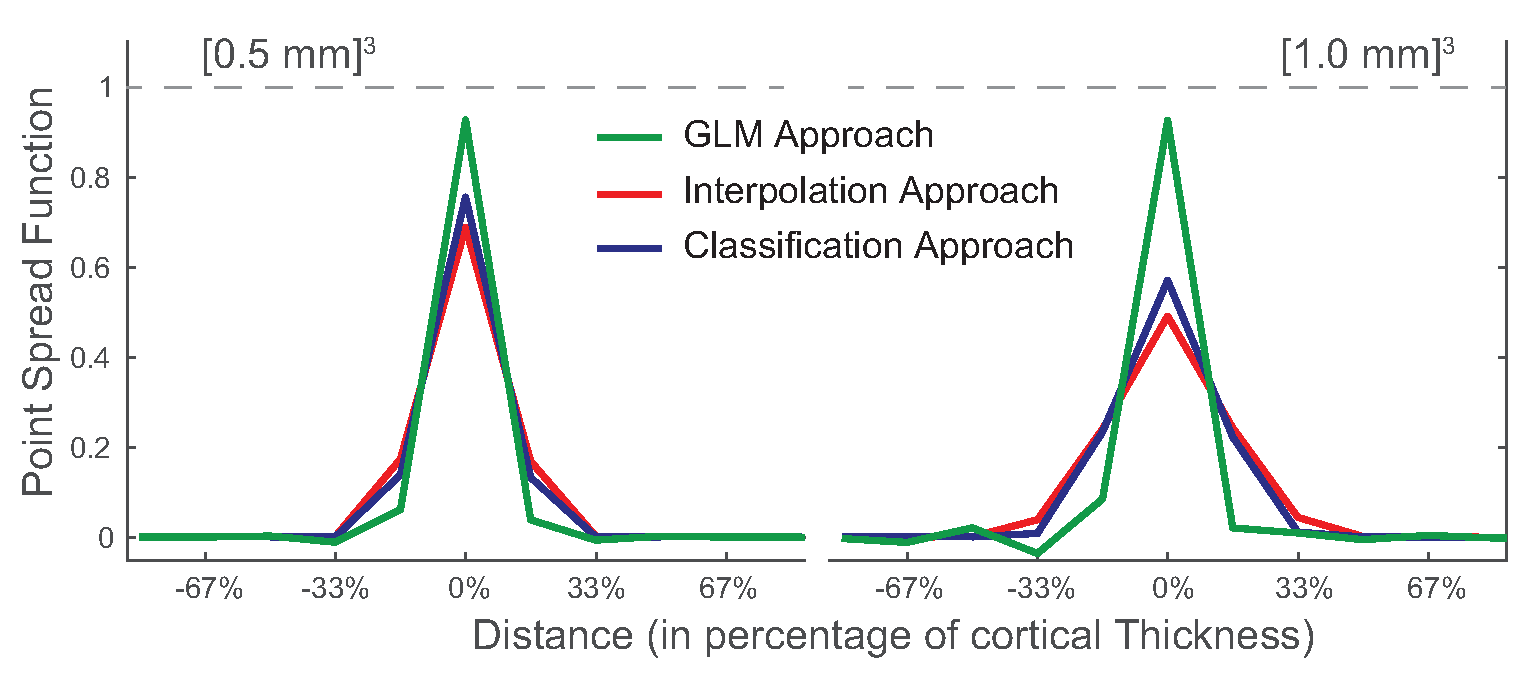
\includegraphics[width=1.\textwidth, clip=true]{./Chapters/03_GLM/./Images/PointSpread}
	\caption{The performance of the three different approaches of obtaining layer signal, represented as a point spread function (PSF) obtained on simulated data. An ideal PSF would be an unit peak at the origin. The results are shown for approximate resolutions of 0.5 mm and 1.0 mm, on the left and right respectively. The GLM approach has a sharper PSF and is able to retrieve more signal, but potentially at the cost of a small undershoot in neighbouring layers.}
	\label{fig:pointspread}
\end{figure}